% don't remove the folling lines, and edit the defintion of \main if needed
\documentclass[../report.tex]{subfiles}
\providecommand{\main}{..}
\IfEq{\jobname}{\currfilebase}{\AtEndDocument{\biblio}}{}
% until here

\begin{document}

\asection[M. Borsato, M. Flechl, S. Gori, L. Zhang]{Searches for beyond the standard model Higgs physics}\label{sec9}
HL and HE-LHC will have an unprecedented opportunity to explore not only the Higgs sector of the SM, but also extended Higgs sectors, as well as rare BSM processes involving the 125 \UGeV Higgs boson. 

In this section, we first discuss the prospects for detecting 125 \UGeV Higgs exotic decays, i.e. decays to light NP particles that eventually decay back to SM particles (Sec. \ref{Sec:9.1Exo}). Higgs exotic decays to collider stable particles (Higgs invisible decays) are already discussed in Sec. \ref{Sec:6Invisible}. Here we report the study of a large array of (semi-) visible decays as $h\to \phi\phi$, where $\phi$ is either a long lived scalar (Secs. \ref{Sec:9.1.1}, \ref{Sec:9.1.2}) or it promptly decays back to two SM fermions (Secs. \ref{Sec:9.1.3}-\ref{Sec:9.1.8}). So far, the LHC has produced $\mathcal O(10)$ million Higgs bosons at its Run 1 and Run 2. This is only $\mathcal O(5\%)$ ($\mathcal O(5\permille)$) the amount of Higgs bosons that will be produced by the HL (HE)-LHC. The huge Higgs statistics that will be collected at the HL/HE-LHC will be a key ingredient for the success of a Higgs exotic decay program. 

In Secs. \ref{sec:Hff}, \ref{sec:XZZ}, we then present the ATLAS and CMS prospects for searching for new heavy Higgs bosons, either in fermionic final states ($H\to\tau\tau$, as particularly motivated in Supersymmetric theories), or in bosonic final states ($H\to ZZ$, as motivated in theories that deviate from the alignment limit). These two sections are followed by a phenomenological section (Sec. \ref{Sec:9.4}) that discusses the reach of possible additional searches for neutral and charged Higgs bosons and the role of interference effects in heavy Higgs searches. The interplay of the 125 Higgs coupling measurements and searches for new degrees of freedom is discussed in Secs. \ref{Sec:9.5}-\ref{Sec:9.7} for several BSM models (the Minimal Supersymmetric SM, Twin Higgs models and composite Higgs models). 

Several well motivated BSM models can also predict new Higgs bosons with a mass below 125 \UGeV. The prospects to probe these light Higgs bosons and the corresponding models are discussed in Sec. \ref{Sec:9.8}. Particularly, light Higgs bosons could be uniquely probed at the HL-stage of the LHCb experiment.


 

%\subfile{\main/section9/mssm_2hdm}

\asubsection{Exotic decays of the 125 \UGeV Higgs boson}\label{Sec:9.1Exo}
\subfile{\main/section9/h4jet}
\subfile{\main/section9/HEHL_HiggsLLP}
\subfile{\main/section9/cms_haa}
\subfile{\main/section9/summary_of_2b2mu}
\subfile{\main/section9/hxswg_curtin_v1}
\subfile{\main/section9/HiggsToALPs}
%Commented out for CDS upload because CMS FTR-18-035 results have not been approved



\asubsection{LHC searches for additional heavy neutral Higgs bosons in fermionic final states}\label{sec:Hff}
\subfile{\main/section9/atlas_htt}
\subfile{\main/section9/cms_htt}


\asubsection{LHC searches for additional heavy neutral Higgs bosons in bosonic final states}\label{sec:XZZ}
%Commented out for CDS upload because CMS FTR-18-040 results have not been approved
\subfile{\main/section9/cms_xzz}

\asubsection{Additional channels for heavy Higgs bosons}\label{Sec:9.4}


%\subsection{Searches for additional Higgs bosons in diboson final states}
% CMS HZZ will be here 


\asubsubsection{Sensitivity to heavy Higgs bosons from the 2HDM in "Higgs-to-Higgs" decays}
\subfile{\main/section9/2HDM_BSM_Higgs_AZH}



\asubsubsection{Interference effects in heavy Higgs searches}\label{Sec.9.4.2}
\subfile{\main/section9/HHinterference}

\asubsubsection{MSSM charged Higgs bosons}
\subfile{\main/section9/MSSMCharged}
%%%%%%%%%%%%%%%%%%%%%%%%%%%%%%%%%%

\subfile{\main/section9/MSSMbenchmarks}
\asubsection{Direct and indirect sensitivity to heavy Twin Higgs bosons}
\subfile{\main/section9/twin_higgs}

\asubsection{Production of $t\bar{t}h$ and $t\bar{t}h h$ at the LHC in Composite Higgs models}\label{Sec:9.7}
\subfile{\main/section9/MCHM_tthh}

%\subsection{Interpretation of the Higgs couplings in terms of Composite Higgs models}
%\subfile{\main/section9/InterpretationCH}







\asubsection{New Higgs bosons below the 125 \UGeV Higgs mass}\label{Sec:9.8}

\asubsubsection[S. Heinemeyer, J. Santiago, R. Vega Morales]{Searches for low mass Higgs bosons (below 120 \UGeV)}

%%%%%%%%%%%%%%%%%%%%%%%%%%%%%%%%%%
\asubsubsubsection{Introduction}

Many extensions of the Standard Model Higgs sector allow for new
charged and neutral Higgs bosons that can be lighter than the Higgs
boson discovered~\cite{Aad:2012tfa,Chatrchyan:2012xdj} at $\approx 125$~\UGeV. 
However, as the observed (heavier) Higgs boson shows itself to be 
increasingly SM-like~\cite{Falkowski:2013dza} in its couplings to $WW$
and $ZZ$ pairs~\cite{Khachatryan:2014kca,Khachatryan:2016vau,Sirunyan:2017exp,Sirunyan:2017tqd,Aaboud:2017oem,Falkowski:2013dza},
as well as to fermions~\cite{Aaboud:2018zhk,CMS:2018abb}, we are in
general pushed into an `alignment without decoupling'
limit~\cite{Gunion:2002zf,Carena:2013ooa}, which has been examined in a
number of recent
studies~\cite{Craig:2013hca,Carena:2014nza,Carena:2015moc,Bernon:2015wef,Profumo:2016zxo,Bechtle:2016kui,Haber:2017erd,Bahl:2018zmf}. In
this limit, the 125~\UGeV Higgs boson has SM like couplings without having
to decouple the other Higgs bosons which might be present allowing them
to be lighter than 125~\UGeV. In what follows we work in the alignment
without decoupling limit focusing on new Higgs bosons in the mass range
$65 - 120$~\UGeV, between the SM-like Higgs mass and its two body decay
threshold. 

In 2HDMs alignment occurs when one of the
neutral CP-even Higgs mass eigen-states is approximately aligned in field
space with the direction of the vacuum expectation value~\cite{Carena:2013ooa,Bernon:2015wef}. For non-doublet
electroweak multiplets (as well as singlets~\cite{Robens:2015gla}), one
obtains an `aligned' SM-like Higgs when the
non-doublet~\cite{Georgi:1985nv,Killick:2013mya} Higgs \emph{VEV} is
small, which typically also suppresses the Higgs mixing
angle~\cite{Haber:1978jt,Hartling:2014zca}. Furthermore, in the singlet
and non-doublet multiplet cases, the new Higgs bosons are (at least
approximately) fermiophobic, making them generically harder to
detect~\cite{Akeroyd:1998ui,Akeroyd:1995hg,Delgado:2016arn,Vega:2018ddp}
either directly or indirectly as we discuss more below.  

In this section we summarise the relevant experimental constraints on
light Higgs bosons in the mass range $65 - 120$~\UGeV. We also discuss
models which can realise light Higgs bosons and highlight promising
search signals at the LHC. This includes searching for deviations in
Higgs couplings since, as emphasised in~\cite{Bernon:2015wef}, even in
the deep alignment regime where one might naively expect everything to
be very SM-like, precise measurements of the 125~\UGeV Higgs boson signal
strengths could uncover the existence of an extended Higgs sector. Some
projections for the HL and HE LHC are also made. 
The aim is to encourage new experimental analysis, targeting
specifically searches for light Higgs bosons at the HL/HE-LHC.

%%%%%%%%%%%%%%%%%%%%%%%%%%%%%%%%%%
\asubsubsubsection{Experimental constraints on light Higgs bosons}\label{sec:limits}


In the mass range and alignment limit we consider, the most relevant
constraints for the \emph{anti}-aligned neutral Higgs bosons but with
significant couplings to SM fermions, come from CMS $b\bar{b}X$ with $X
\to \tau\bar{\tau}$ searches~\cite{Khachatryan:2015baw} as well as
ATLAS~\cite{Aad:2014vgg} and CMS~\cite{Khachatryan:2014wca} searches for
$X \to \tau\bar{\tau}$ decays in both the $gg \to X$ and $b\bar{b}X$
production modes. Similarly, the searches in the di-photon channel
  place important bounds~\cite{CMS-PAS-HIG-17-013,ATLAS-CONF-2018-025}.%
\footnote{It is interesting to note that the CMS search in the di-photon
  channel~\cite{CMS-PAS-HIG-17-013} shows an excess of events at $\sim
  96$~\UGeV, in the same mass range where the LEP searches in the 
  $b \bar b$ final state observed a $2\,\sigma$ excess~\cite{Schael:2006cr}.}
A recent CMS search~\cite{CMS:2015mba} for new
resonances decaying to a $Z$ boson and a light resonance, followed by 
$Z \to \ell\bar\ell$ and the light resonance decaying to $b\bar{b}$ or
$\tau\bar{\tau}$ pairs, has also been shown to impose severe
constraints~\cite{Bernon:2015wef} on light CP-even neutral Higgs
bosons. Direct searches at LEP for light neutral Higgs states produced
in pairs or in association with a $Z$ boson are also
relevant~\cite{Barate:2003sz,Abbiendi:2004gn,Schael:2006cr},
setting relevant limits on the couplings of the light Higgs to SM
gauge bosons. For
the charged Higgs bosons, LEP searches~\cite{Abbiendi:2013hk} and
$B$-physics constraints from $R_b,\,\epsilon_K,\,\Delta m_B,\,B\to
X_s\gamma$, and
$B\to\tau\nu$~\cite{Haisch:2008ar,Mahmoudi:2009zx,Gupta:2009wn,Jung:2010ik,Misiak:2015xwa}
measurements impose the most stringent constraints. These limits apply
to all 2HDMs and impose particularly severe constraints on
\emph{non}-type-I 2HDMs~\cite{Bernon:2015wef} in which there is no
fermiophobic limit.  

As emphasised in numerous studies~\cite{Ilisie:2014hea,Enberg:2016ygw,Delgado:2016arn,Degrande:2017naf,Vega:2018ddp}, the above limits are less stringent (most limits can be rescaled) when the Higgs bosons have highly suppressed couplings to SM fermions as can happen in the type-I 2HDM~\cite{Haber:1978jt} in the large $\tan\beta$ limit~\cite{Akeroyd:1995hg}. For non-doublet extended Higgs sectors one automatically has suppressed couplings to SM fermions when the non-doublet \emph{VEV} is small (or mixing angle in the case of singlets) since they only enter (if at all) through mixing with the SM-like Higgs boson~\cite{Killick:2013mya}.~In the case of fermiophobia, the most robust probes of neutral Higgs bosons are inclusive di-photon~\cite{Delgado:2016arn,Degrande:2017naf,Vega:2018ddp} and multi-photon searches~\cite{Akeroyd:2005pr,Abdallah:2003xf,Aaltonen:2016fnw} which utilise the Drell-Yan pair production channel of a charged and neutral Higgs boson.~Constraints from EW precision data~\cite{Baak:2011ze,ALEPH:2010aa} also apply with the primary effect being that the neutral and charged Higgs bosons are constrained to be not too different in mass.  

%%%%%%%%%%%%%%%%%%%%%%%%%%%%%%%%%%
\asubsubsubsection{Models with light Higgs bosons}\label{sec:models}

A number of recent studies of the alignment without decoupling limit in
2HDMs have been performed which consider the case where the SM-like
Higgs boson is not the lightest scalar. As shown
in~\cite{Ilisie:2014hea,Bernon:2015wef,Enberg:2016ygw,Arhrib:2017wmo,Arbey:2017gmh,Bhatia:2017ttp,Fox:2017uwr,Haber:2017erd,Haisch:2017gql},
for type-I 2HDMs there are regions of parameter space where, along with
the light CP-even scalar, both the charged and neutral CP-odd Higgs
bosons can be below the SM-like Higgs mass while satisfying the
constraints discussed above. This is in contrast to type-II 2HDM,
where combined constraints from $B$ meson
decays~\cite{Misiak:2015xwa} and EW precision
constraints~\cite{Peskin:1991sw} require the charged and CP-odd neutral
Higgs bosons to be much heavier than the mass range we consider here. Within the MSSM however, the additional particle content results in
  substantially weaker limits from $B$~meson decays and EW data.
In general the allowed regions of parameter space in the type-I 2HDM is
much larger than in other 2HDMs~\cite{Bernon:2015wef,Haber:2017erd},
again due to the presence of a fermiophobic limit at large $\tan\beta$
which opens up more regions of parameter space. 

In the MSSM which is a type-II 2HDM, the alignment without decoupling
limit~\cite{Carena:2013ooa} requires accidental cancellations between
tree level and radiative corrections in the Higgs mass
matrix~\cite{Bechtle:2016kui,Haber:2017erd}. It was shown that a tuning of $\sim 10\%$ is sufficient to find agreement with the Higgs-boson rate measurements~\cite{Bechtle:2016kui}. Depending on the level of alignment required, this can lead to a highly constrained parameter space, especially in the case where the SM-like Higgs is the heavier of the CP-even neutral scalars. In particular, after accounting for all relevant experimental constraints (as well as theoretical uncertainties) recent studies~\cite{Bahl:2018zmf} of the alignment without decoupling limit of the MSSM~\cite{Carena:2013ooa} defined a benchmark plane of allowed parameter space with $\tan\beta \sim 5 - 6$ (and very large values of $\mu$) in which the light CP-even Higgs can be between  $\sim 60 - 100$~\UGeV if the charged Higgs mass is between $\sim 170 - 185$~\UGeV and the neutral CP-odd Higgs is $\sim 130 - 140$~\UGeV. Still larger allowed regions are expected in a global scan, as performed in~\cite{Bechtle:2016kui}.
Recent studies of the NMSSM~\cite{Carena:2015moc,Domingo:2018uim} and
$\mu\nu$SSM~\cite{Biekotter:2017xmf} have also examined the alignment
without decoupling limit finding a larger allowed parameter space than in the
MSSM due to an additional gauge singlet Higgs (or right handed scalar
neutrino). 

For models with non-doublet multiplets the most well known are those involving electroweak triplets. In particular, Higgs triplet models with custodial symmetry~\cite{Sikivie:1980hm}, as in the famous Georgi-Machacek (GM) model~\cite{Georgi:1985nv,Chanowitz:1985ug,Gunion:1989ci,Gunion:1990dt,Hartling:2014zca} or its supersymmetric incarnations~\cite{Cort:2013foa,Garcia-Pepin:2014yfa,Vega:2017gkk}, have been well studied due to their ability to easily satisfy constraints from electroweak precision data. Recent studies~\cite{Davoudiasl:2004aj,Vega:2017gkk,Vega:2018ddp} have shown that GM-like models can allow for light neutral and charged scalars below the SM-like Higgs boson mass. In the alignment limit implied by Higgs coupling measurements, the triplet Higgs \emph{VEV} is constrained to be small though it can still much larger than non-custodial cases~\cite{Tanabashi:2018oca,Haber:1999zh} which are constrained by measurements of the $\rho$ parameter. Custodial symmetry also ensures that the neutral and charged components of the Higgs multiplet have (at least approximately) degenerate masses, making them more difficult to detect due to soft decay products~\cite{Buckley:2009kv,Ismail:2016zby}. For these anti-aligned and fermiophobic Higgs bosons, recent studies have emphasised di- and multi-photon searches~\cite{Aaltonen:2016fnw,Delgado:2016arn,Brooijmans:2016vro,Vega:2018ddp} as robust probes of this scenario.

%%%%%%%%%%%%%%%%%%%%%%%%%
\asubsubsubsection{Phenomenology of light anti-aligned Higgs bosons}\label{sec:pheno}

In the alignment limit, single electroweak production mechanisms for the
additional `anti-aligned' neutral Higgs bosons (or small \emph{VEV} and Higgs mixing for non-doublets), such as VBF or associated vector boson production, necessarily become suppressed. Thus the dominant production mechanisms become gluon fusion or associated $b\bar{b}$ production when there is a significant coupling to SM quarks. However, these production mechanisms become suppressed when the couplings to fermions are negligible\,\footnote{Of course if they couple to some not too heavy coloured BSM particles, the gluon fusion cross section can be increased.}, as can happen in type-I 2HDM in the large $\tan\beta$ limit~\cite{Akeroyd:2003bt} or non-doublet electroweak sectors which are generically fermiophobic. The same is true for the light charged Higgs bosons production channels $t \to H^\pm b$ and $pp \to H^\pm t b$ which are also obsolete in the fermiophobic limit. Note that for charged scalars coming from larger than doublet representations we can also have $W^\pm Z \to H^\pm$ VBF production, but this is again suppressed in the small non-doublet \emph{VEV} and Higgs mixing limit. 


%%%%%%%%%%%%%%%%%%%%%%%%%
{\bf{Pair Production as a discovery channel}}\label{sec:pair}

A different option that offers new experimental opportunities is
  the Drell-Yan Higgs pair production mechanism. Any extension of the SM Higgs sector by electroweak charged scalars will possess the pair production channels mediated by $W$ and $Z$ bosons and which are not present in the SM. Furthermore, as emphasised in~\cite{Akeroyd:2003bt,Akeroyd:2003xi,Akeroyd:2003jp,Ilisie:2014hea,Delgado:2016arn,Vega:2018ddp}, even in the alignment and fermiophobic limits, this production mechanism is not suppressed and can be as large as $\sim 10\,pb$ at 13~\UTeV and $\sim 50\,pb$ and 27~\UTeV in the mass range we consider (see Sec.~\ref{sec2_HXSWG1}). Thus, Drell-Yan Higgs pair production can be as large or even dominate over single  production mechanisms, for both charged and neutral Higgs bosons. Despite this, the Drell-Yan Higgs pair production mechanism has been largely overlooked in experimental searches with the lone exception being a recent CDF analysis of Tevatron four photon data~\cite{Aaltonen:2016fnw} searching for fermiophobic Higgs bosons.  

The Drell-Yan pair production mechanism is mediated by the vector-Higgs-Higgs coupling. In the alignment limit, this will have vertices that are maximised in this limit and depend only on electroweak couplings and quantum numbers, while some vertices will go to zero depending on which Higgs pairs are being produced~\cite{Akeroyd:2003bt,Akeroyd:2003xi,Akeroyd:2003jp,Ilisie:2014hea,Delgado:2016arn,Vega:2018ddp}. Thus for the non-zero cases the coupling can be written schematically as,
%
\bea\label{eqn:gvhh}
g_{WH_M^\pm H_N^0} \equiv i g 
\, C_N (p_1 - p_2)^\mu ,~~
g_{ZH_M^0H_N^0} \equiv i \frac{g}{c_W} 
\, C_N (p_1 - p_2)^\mu ,
\eea
%
where $C_N$ is fixed by the $SU(2)_L\times U(1)_Y$
representation~\cite{Georgi:1985nv,Akeroyd:2003bt,Akeroyd:2010eg,Cort:2013foa,Hartling:2014zca} and $p_{1}, p_{2}$ are the four momenta of the incoming and outgoing scalar momenta. Here $H_N^0$ stands for any neutral Higgs boson and can include CP-even or CP-odd neutral Higgs bosons, as well as $H_M^\pm$ charged Higgs bosons. There is also a photon mediated channel when both Higgs bosons are charged, but we focus on cases where at least one is neutral. In Fig.~\ref{fig:HHprod} we show the leading order $q\bar{q} \to V \to H_M^{\pm,0} H_N^0$ (including \emph{PDFs}) cross section $\times\, C_N^{-2}$ for the $W$ mediated (blue solid) and $Z$ mediated (black dashed) channels at the LHC with $\sqrt{s}=13$~\UTeV (left) and $\sqrt{s}=27$~\UTeV (right) in the mass range $60 - 125$~\UGeV. They are computed with Madgraph~\cite{Alwall:2014hca} using a modified version of the GM model implementation of~\cite{Hartling:2014xma} and rescaling appropriately. There are also NLO contributions which may generate $\gtrsim \mathcal O(1)$ K-factors for Higgs pair production~\cite{Eichten:1984eu,Dawson:1998py,Degrande:2015xnm}. These are not included in our analysis. We show four cases for mass splittings  of $\Delta M \equiv M_{H^{\pm,0}_M} - M_{H_N^0} = 0, 100, 200, 300$~\UGeV as labelled in plot.  
%%%%%
\begin{figure}[tbh]
\begin{center}
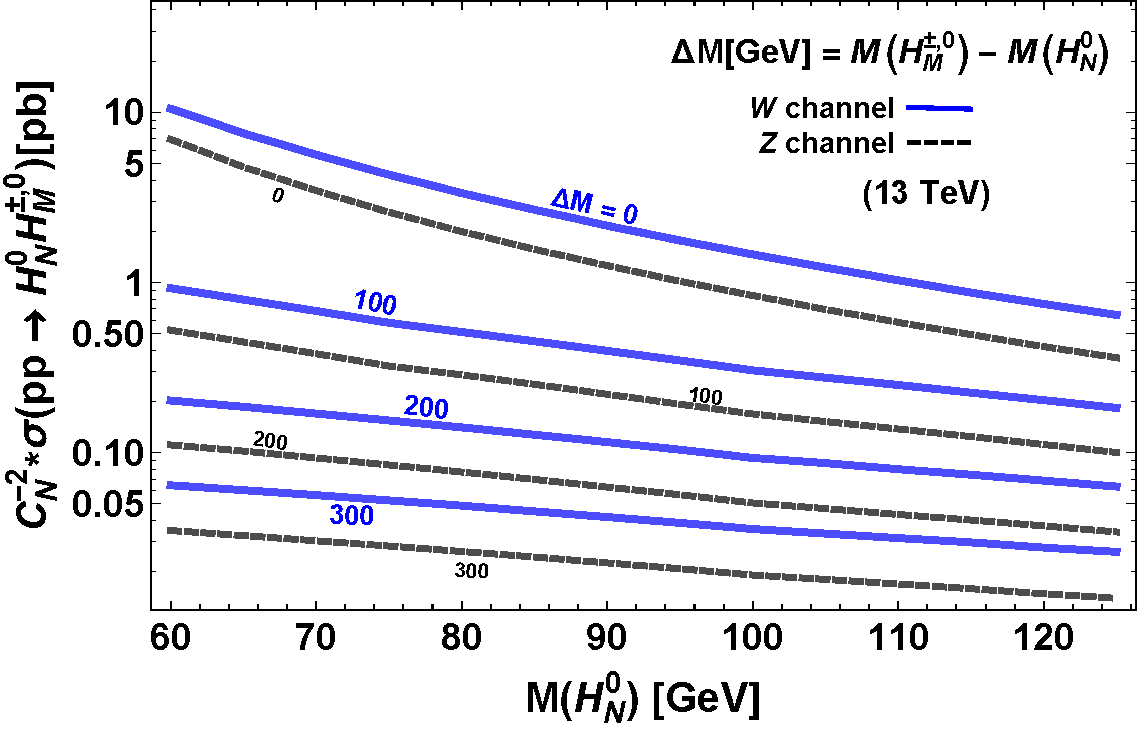
\includegraphics[scale=.403]{\main/section9/plots/CxnVsMHoDelM_13TeV.pdf}
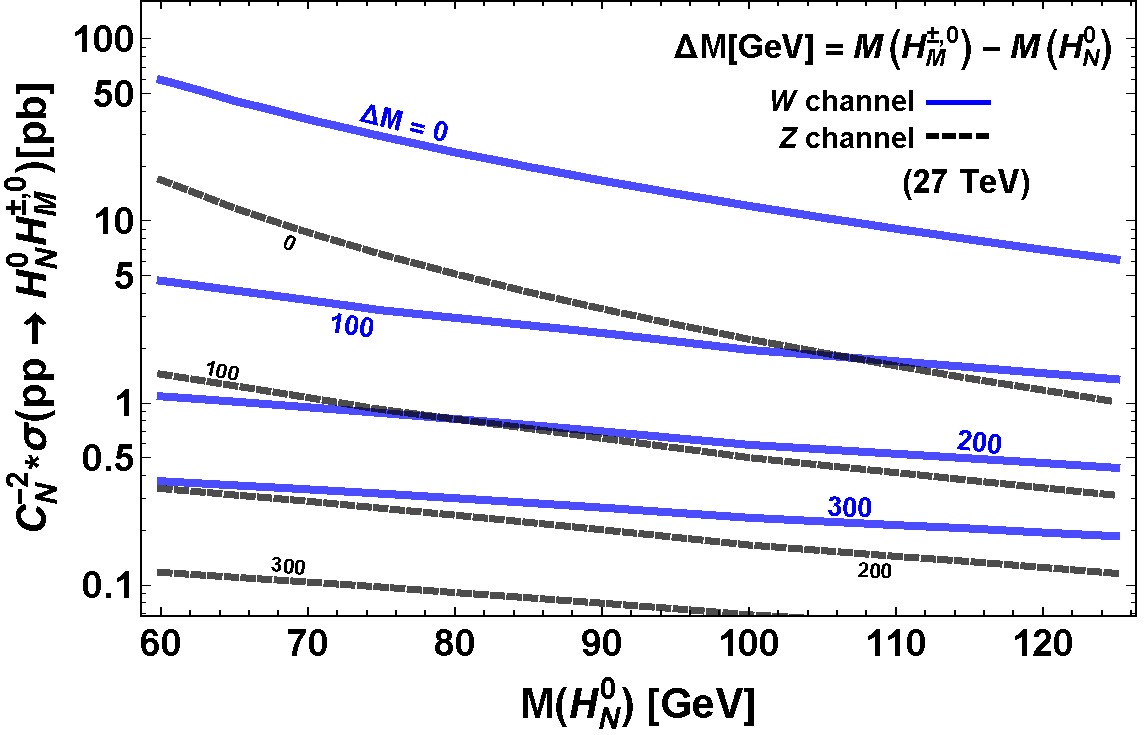
\includegraphics[scale=.4]{\main/section9/plots/CxnVsMHoDelM_27TeV.pdf}
\end{center}
\caption{Leading order cross sections (with \emph{PDFs}) for the $q\bar{q} \to V \to H_M^{\pm,0} H_N^0$ Higgs pair production mechanism mediated by $W$ (blue solid) and $Z$ (black dashed) bosons at the LHC for $\sqrt{s}=13$~\UTeV (left) and $\sqrt{s}=27$~\UTeV (right) in the mass range $60 - 125$~\UGeV. We show three cases for mass splittings $\Delta M \equiv M_{H^{\pm,0}_M} - M_{H_N^0}= 0, 100, 200, 300$~\UGeV as labelled in plot and have factored out an overall group theory factor $C_N$ (see Eq. (\ref{eqn:gvhh})). The curves for a particular model can be obtained by rescaling with $(C_N)^2$ which is fixed by the $SU(2)_L\times U(1)_Y$ representation.} 
\label{fig:HHprod}
\end{figure}
%%%%%

The dominant decay modes of the neutral Higgs bosons will be to $b\bar{b}$ and $\tau\bar{\tau}$ when there is a significant coupling to SM fermions. In the fermiophobic case, the Higgs bosons can have large branching ratios into EW gauge bosons and in particular photons at low masses. The less emphasised $Z\gamma$ channel may also offer promising opportunities~\cite{Degrande:2017naf}. Inclusive searches for resonances can then be combined with the Drell-Yan production channel to put relatively robust bounds on branching ratios in extended Higgs sectors as done in~\cite{Delgado:2016arn,Vega:2018ddp} for the case of decays into di-photons. For the charged Higgs bosons combing Drell-Yan pair production with decays into $W\gamma$~\cite{Ilisie:2014hea,Degrande:2017naf} or four photon signals~\cite{Aaltonen:2016fnw} offer promising search channels.


%%%%%%%%%%%%%%%
{\bf{Suggestions for searches at the HL/HE-LHC}}

We briefly summarise search strategies for (anti)-aligned light
Higgs bosons at the (HL/HE) LHC to be added to the current searches in the mass range we consider, including
$\tau\tau,\,\gamma\gamma,\,b\bar{b}$ searches based on gluon fusion and
$\tau\tau$ searches based on associated $b\bar{b}$
production~\cite{Aad:2014vgg,Khachatryan:2014wca,Khachatryan:2015baw} as
well as recent CMS searches~\cite{CMS:2015mba} for $A \to Zh$ with $Z
\to \ell\bar\ell$ and $h\to \tau\tau, bb$.  

%%%%%%%%%%%%%%%%
%\subsection{Suggestions for searches at the HL/HE-LHC}

\begin{itemize}
\item Push current conventional Higgs searches in $WW$ and $ZZ$, which
  currently~\cite{Khachatryan:2015cwa,Sirunyan:2018qlb} do not go below
  $\sim 130$~\UGeV, to as low a mass as possible, ideally down to $\sim
  65$~\UGeV. As emphasised in~\cite{Delgado:2016arn,Vega:2018ddp}, this
  can help to rule out cases of a fermiophobic Higgs boson with
  suppressed couplings to photons, which could otherwise escape
  detection. Similarly, heavier Higgs bosons with the ``remaining''
  coupling to SM gauge bosons could be detected.

\item Combine \emph{inclusive} searches for resonances with the
  `universal' Drell-Yan Higgs pair production channel to put robust
  bounds on allowed branching ratios to $\tau\tau$, $b\bar{b}$, $Z\gamma$ and
  $\gamma\gamma$ final states. In the alignment limit,
  these bounds depend only on electroweak couplings and can be applied
  to any extended Higgs boson sector (with appropriate rescaling), in
  some cases providing the strongest limits~\cite{Delgado:2016arn,Vega:2018ddp}.

\item Utilising the Drell-Yan Higgs pair production mechanism, dedicated
  LHC searches for more optimised, but model dependent signals such as
  $4\gamma + V^\ast$~\cite{Akeroyd:2003bt,Aaltonen:2016fnw,Arhrib:2017wmo},
  $4\gamma + V^\ast V^\ast$~\cite{Akeroyd:2003bt}, $3\gamma +
  V^\ast$ where in the last case dedicated phenomenological studies are
  lacking. 

\item Search for $\tau\tau$, $b\bar{b}$, or $\gamma\gamma$ plus missing
  energy as well as mono photon or mono lepton plus missing energy final
  states to cover cases where neutral Higgs may have an invisible
  decay. In particular the $\gamma\gamma$ channel appears to be
  very promising (especially in view of a potential signal at 
  $\sim 96$~\UGeV~\cite{CMS-PAS-HIG-17-013}).
 
\end{itemize}

\asubsubsection{HL-LHC projections of LHCb searches for 2HDM+S light pseudoscalars}\label{Sec:9.8LHCb}
\subfile{\main/section9/lhcb}

%\bibliography{\main/section9/bib/section.bib}

\end{document}
